\begin{figure}
%	\setlength\abovecaptionskip{0.5\baselineskip}
%  	\setlength\abovecaptionskip{0.75\baselineskip}
        \begin{center}
    		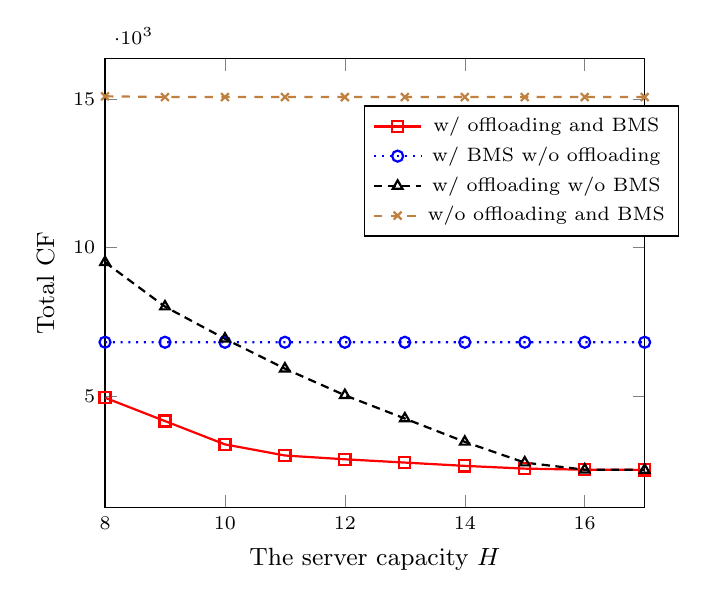
\begin{tikzpicture}
        		\begin{axis}[
        		%	scaled ticks=true, 
        		%	scaled y ticks={real:1e3},
        			scaled y ticks=base 10:-3,
        		    %title={},
        		    xlabel={The server capacity $H$},
        		    ylabel={Total CF},
        		    xmin=8, xmax=17,
        		  %  ymin=0, ymax=3500,
        		  %  xtick={25, 50, 75, 100, 125, 150},
        		%	xticklabels=\empty,
        %		    ytick={0, 1000, 2000, 3000},
        		%	point meta=y *10^3, % the displayed number
        		  %  legend pos=north east,
        		    legend style={at={(0.48, 0.75)},anchor=west},
        		    %ymajorgrids=true,    
        		    %xmajorgrids=true,
        		    grid style=densely dashed,
        		    tick label style={font=\scriptsize},
        		    label style={font=\small},
        		    legend style={font=\scriptsize},
        		]
        		
            		\addplot[ color=red, mark=square, line width=0.8pt]     
            		coordinates { 
                    ( 8 , 4949.3 )
                    ( 9 , 4163.9 )
                    ( 10 , 3379.7 )
                    ( 11 , 3005.4 )
                    ( 12 , 2878.1 )
                    ( 13 , 2767.4 )
                    ( 14 , 2656.7 )
                    ( 15 , 2564.0 )
                    ( 16 , 2528.3 )
                    ( 17 , 2521.1 )
            		};
            		%
            		\addplot[ color=blue, mark=o, dotted, mark options={solid}, line width=0.8pt]     
            		coordinates {
                    ( 8 , 6818.0 )
                    ( 9 , 6816.0 )
                    ( 10 , 6815.0 )
                    ( 11 , 6815.0 )
                    ( 12 , 6815.0 )
                    ( 13 , 6815.0 )
                    ( 14 , 6815.0 )
                    ( 15 , 6815.0 )
                    ( 16 , 6815.0 )
                    ( 17 , 6815.0 )
            		};
            		
            		\addplot[ color=black, mark=triangle, densely dashed, mark options={solid}, line width=0.8pt]
            		coordinates {
                    ( 8 , 9506.6 )
                    ( 9 , 8014.9 )
                    ( 10 , 6933.3 )
                    ( 11 , 5927.9 )
                    ( 12 , 5033.1 )
                    ( 13 , 4248.9 )
                    ( 14 , 3464.7 )
                    ( 15 , 2766.0 )
                    ( 16 , 2528.3 )
                    ( 17 , 2521.1 )
            		};
            		
            		\addplot[ color=brown, mark=x, dashed, mark options={solid}, line width=0.8pt]
            		coordinates {
                    ( 8 , 15091.0 )
                    ( 9 , 15065.0 )
                    ( 10 , 15065.0 )
                    ( 11 , 15065.0 )
                    ( 12 , 15065.0 )
                    ( 13 , 15065.0 )
                    ( 14 , 15065.0 )
                    ( 15 , 15065.0 )
                    ( 16 , 15065.0 )
                    ( 17 , 15065.0 )
            		};

            		\legend{w/ offloading and BMS, w/ BMS w/o offloading, w/ offloading w/o BMS, w/o offloading and BMS}
        		
        		\end{axis}
    		\end{tikzpicture}
    		
        \end{center}
    \caption{Caption.}\label{fig:result3}
\end{figure}
